% Copyright (c) 2014,2016 Casper Ti. Vector
% Public domain.

\chapter{绪论}

\section{背景知识和研究意义}

随着网路技术的迅猛发展,大量的信息需要通过网络进行交互,在其给人们带来巨大便利的同时,也存在着巨大的安全隐患。在网络中传输的数据可能会被恶意的攻击方非法的窃听,导致传输信息的泄露,如何保证数据在传输过程中的机秘密性、完整性和不可否认性一直是网络安全技术所关注的问题,而公钥基础设施PKI(Public Key Infrastructure)技术是解决这一问题的重要手段.


公钥基础设施PKI作为利用非对称加密算法原理和技术实现并提供安全服务的技术和规范,已经成为互联网中保证数据传输保密性、完整性和不可否认性的重要组成部分。PKI体系中的证书,已经被广泛地应用在各种身份认证的场景下,特别是在互联网中建立SSL通信的过程中,用于保证客户端对服务器身份的认证。


证书在PKI系统中作为公钥和标识绑定的载体,起着流通信任的作用。围绕证书而言,在该系统存在的角色主要包括以下三类:授权机构(CA),用户以及依赖方。在PKI系统中,用户发起证书签发请求,递交给授权机构;授权机构负责证书的签发吊销等管理工作;依赖方则是证书的受用对象,检查证书的合法性并从中获得对方的公钥。

证书是否有效是通过验证该证书是否由授权机构所签发来决定的。依赖方会事先将所有授权机构的相关证书下载到本地,在通信过程中获取对方证书和证书链来验证证书的有效性;而证书附有公钥和标识的绑定关系,之后会用该公钥与对方进行通信,并认为拥有对应私钥的人就是绑定标识者。也就是说,授权机构是整个系统中的信任支点,系统中的依赖方需要对其签发的证书给予绝对信任。如果授权机构有作恶行为,比如签发虚假的证书,网络中的实体并不能辨认该证书的真伪,导致系统中的依赖方与虚假的身份进行通信。

在现有的PKI系统中,授权机构和用户之间的权利是不对等的,用户只能发起证书签发请求,而不能对授权机构是否签发证书起到制约性。由于信任都集中在中心化的授权机构之上,恶意的授权机构或者被攻破的授权机构将可以签发任意用户的证书,从而对相应用户发起中间人攻击,对整个系统带来恶劣的影响。比如在2011年,DigiNotar遭到入侵,签发的虚假证书涉及到20多个网域的200多个SSL证书\supercite{prins2011diginotar},对用户造成了巨大影响,最终导致自身被吊销授权机构资格的后果。

由于授权机构以中心化的形式存在于PKI系统中,并受到了所有实体的绝对信任,一旦其出现问题那么将会瓦解整个信任体系。为了防止授权中心的不端行为,如何去平衡PKI系统中实体的权利一直都是大家说关注的问题。如果授权中心在签发证书前也需要用户同意,那么将会大大减小授权中心被攻破或有不端行为所带来的影响。

区块链作为比特币底层的核心技术,具有去中心化、防篡改的特性,使得比特币与传统货币相比无需信任中心,不依赖第三方来保证其上交易过程的安全性。比特币由于不需要中心化的发行机构,不会被组织或政府操控的特性,受到大家的广泛关注。从最初的类似比特币这样的密码货币争相发布,到现在与区块链相关的传统应用出现在大家的视野中,区块链技术逐渐的被应用在其它领域,其去中心化、防篡改的特性成为了这些应用的核心所在。

如前面所说的那样,PKI中授权中心和用户之间权利不对等,如何去减弱用户对授权中心的依赖十分重要。而区块链技术作为应用在P2P网络中的底层技术,可以在无需中心的情况下,完成对网络中事务的状态统一,保证该网络中实体的各自权益对等。区块链的这些特性可以借鉴并应用到PKI系统中,解决PKI中实体之间的权利不对等所带来的安全隐患,巩固PKI系统的安全。


\section{国内外研究现状}

\subsection{PKI的研究现状}

1976年,美国密码学专家Diffie和Hellman提出了著名的D-H密码分发体制,从而解决了不使用秘密信道进行密钥分发的问题,允许通信双方可以在不安全的通信线路上完成密钥信息交换。在1978年,CA认证中心由Kohnfelder提出,在他给出的方案中,CA集中式的管理公钥,以CA证书的形式公布于目录库中,私钥继续使用秘密信道分发。1996年PKI的解决方案被正式提出,PKI设立CA认证中心,以第三方权威机构的身份完成对公钥和标识的绑定。

经过二十多年的发展,PKI作为提供信息安全服务的基础性普适性设施,无论在理论上还是技术上,都已经日趋成熟。在理论方面,以公钥密码学作为基础的密码算法、协议以及认证方法都得到了全面的发展,为PKI技术提供了安全性保障;在技术上,数字证书的申请、签发和管理,数字证书的相关应用格式,以及PKI实体之的通行协议都被相继提出并制定,使得PKI技术可以按照相应的标准使用在一系列的场景之下。


由于公钥基础设施PKI的存在,我们可以安全地与仅拥有对方公钥的人进行安全通信,通过信任第三方机构CA签发的证书完成公钥与身份的绑定。从安全的角度去审视现有的Internet PKI生态系统,主要存在以下几个方面的问题:首先,最为严重的问题是CA拥有绝对的权利,在未经实体允许的情况下就可以给其签发证书;其次,对CA的信任是没有灵活度的,只存在信任与否的抉择;其三是在域名证书的验证过于薄弱,在传统的方法中只是进过简单的邮箱确认方式,并不是特别安全;最后是证书的吊销不能正常工作,在很多实际使用的情况下,对证书吊销的检查并不完整\supercite{ristic2014bulletproof}。

如上所提及的那样,对CA的信任是绝对的,而且CA拥有绝对有的权利,单个恶意或者被攻破的CA可以给任意一个域名签发证书\supercite{ducklin2013turktrust};同时对于该类假冒的证书,将会需要很大一段时间才能被发现。我们知道全球存在很多很多的CA,不同CA的安全防护能力各不相同,攻击者只需要攻破单个CA,即可签发任意域名的假冒证书,从而对该域名发起中间人攻击,达到攻击相关域名的目的。





%From evaluate web PKI
%calss one Difference observation
为了检测通信过程中的证书是否可靠,一些列方案通过依赖方在浏览器端询问不同的证书提供者,对比得到的多个证书信息的一致性来确保证书的有效性。Perspectives\supercite{wendlandt2008perspectives}在2008年被Wendlant等人提出,并通过插件的方式应用于FireFox之上,该方案通过在建立安全连接前询问不同的公证服务器来检测该域名的公钥是否合法,一旦发现得到的密钥不相同,将检测出是否有人发起了中间人攻击(MITM)。然而由于证书的传播需要时间,对于新签发的证书可能需要一段时间才可以使用以上的服务,二次验证\supercite{alicherry2009doublecheck}的方案在09年被提出,该方案的主要思路是向目标服务器请求两次证书:一次通过TLS连接,另外一次使用Tor\supercite{alicherry2009doublecheck};该方法在一定程度上同时解决了浏览器泄露用户隐私的问题。另外一个Perspectives存在的问题是用户向其请求证书的同时,暴露了自己访问的历史记录,泄露了自身的隐私。为了解决这一问题,Convergence\supercite{convergence}的方案被提出,在用户向公证服务器请求证书的时,将不是直接向某一公证服务器请求数据,而是随机的选择一个公证服务器将其请求转发给其它公证服务器,类似洋葱路由的机制。

\renewcommand\arraystretch{2}
\begin{table}[h]
\centering
\begin{tabular}{p{2.5cm}p{12cm}}
	\hline
	分类 & 存在的方案 \\
	\hline
	传统 & \small 基于CA的证书管理系统 \\
	\hline
	\multirow{2}{*}{证书验证} & \small Perspectives ('08)\parencite{wendlandt2008perspectives}; 二次验证('09)\parencite{alicherry2009doublecheck};   \\ \cline{2-2}
	& \small Convergence('11)\parencite{convergence}; Certificate Patrol('11)\parencite{modell2014certificate}; CertLock('11)\parencite{soghoian2011certified}; TACK('12)\parencite{marlinspike2012internet} \\
	\hline
	签发限制 & \small HPKP('11)\parencite{evans2015public}; DANE('11)\parencite{barnes2011dane}; CAGe('13)\parencite{kasten2013cage} \\
	\hline
	\multirow{2}{*}{签发审计} & \small Sovereign Keys('12)\parencite{eckersley2012internet};Certificate Transparency('12)\parencite{laurie2013certificate}; \\ \cline{2-2}
	& \small AKI('13)\parencite{kim2013accountable}; CIRT('14)\parencite{ryan2014enhanced}; ARPKI('14)\parencite{basin2014arpki}; DTKI('14)\parencite{cheval2014dtki}	 \\
	\hline
	
\end{tabular}
\caption{存在的解决方案}\label{proposed} %显示表格的标题  
\end{table}

由于证书的有效期一般相对比较长,当一个新的证书被使用时,很有可能它是攻击者伪造的证书并发起了攻击,基于这一点Certificate Patrol\supercite{modell2014certificate}的方法在检测到新证书时会向用户发起提示;同时,一般情况下证书的申请也会向自己国家的授权机构发起,当得到一个其它国家的签发的证书时,同样很有可能是虚假的证书,CertLock\supercite{soghoian2011certified}就是基于这个想法而提出的方案。%TACK方案XXX



%class two Scope restriction
一些方案希望通过域名或其它的限制来削弱CA的权利,HPKP\supercite{evans2015public}就是其中的一种。HPKP 技术给予域名主动选择信任 CA 的权利,它的工作原理是通过响应头或者 <meta> 标签告诉浏览器当前网站的证书指纹,以及过期时间等其它信息。DANE\supercite{barnes2011dane}方案则希望借助DNSSEC来发布域名相关的公钥信息;也就是说,域名可以将其公钥保存在DNS记录中,当浏览器发起DNS解析服务的时候,就能够获取到相应域名所使用的公钥信息,并用于验证收到证书的正确性当中。
CAge方案则和CertLock拥有类似的出发点,通过在客户端浏览器上给各个CA设定允许签发服务器证书的顶级域名范围,来保证CA不能随意的去签发证书,一定发现其签发了范围之外的服务器证书,则会向用户发起警告提示。
CAge方案通过在客户端浏览器上给各CA 设定所允许签发服务器证书的顶级域名范围; 一旦发现有 CA 签发了设定范围之外的服务器证书, 则警告提示用户
%CAgeXXX

%class threre Certificate management transparency
另外一些方案旨在让CA的行为变得更加透明,基本的想法是使用公共的日志来完成对证书签发的记录,从而利益相关方可以检查这些日志,查看是否存在错误签发的证书。Soveregin Keys(SK)\supercite{eckersley2012internet}是第一个使用公共日子服务器的PKI方案。在该方案中,允许域名拥有者宣称一个长期的主权密钥,该密钥存储在一个公共的只增服务器上,并提供多个镜像服务器供公众访问。当浏览器在建立安全连接之前,需要检查使用的证书是否被主权公钥签名,验证失败的情况下将不会建立连接。

Certificate Transparency(CT)\supercite{laurie2013certificate}是由Goole提出的另外一种方案,旨在帮助域名拥有者检测错误签发的证书。该方案中要求CA签发证书的操作都要记录在公开可审计的日志服务器上,未被记录的证书将得不到认可。证书透明的方案并没有考虑到证书吊销的问题,Certificate Issuance and Revocation Transparency(CIRT)\supercite{ryan2014enhanced}方案在证书透明的基础上加入了证书吊销相关的审计服务,在日志服务器能够上维护可审计的证书撤销状态信息。更进一步,Distributed Transparent Key Infrastructure(DTKI)\supercite{cheval2014dtki}方案作为CIRT的改进,通过设置两种不同类型的日志服务器,来减弱对CIRT中单类型日子服务器的信任,使得其具有更高的安全性。


与SK方案相似,Accountable Key Infrastructure(AKI)\supercite{kim2013accountable}也允许域名拥有者去申明证书相关的规则,比如哪些CA或者日志维护者可以为其提供服务、证书中至少需要包含多少个签名等的策略。这样更加进一步限制了PKI系统中单个实体的权利,不会因为系统中的单个CA的疏忽或者不端行为造成虚假证书的流通。Attack Resilient Public-Key Infrastructure(ARPKI)\supercite{basin2014arpki}作为AKI的改进方案被随后提出,相比于AKI,该方案在建模过程中加入了安全性验证,理论上具有更好的安全特性。





%
%(换一种形式)	
%为了加强X.509 PKI体系的安全性并减弱对单个CA的信任,各种方案被提出来,根据PKI中存在的不同实体类型可分为以客户端为中心的方法、以CA为中心的方法和以域名为中心的方发。以客户端为中心的方法重点放在在客户端接受证书前对证书的评估,例如Policy engine\supercite{abadi2013global}、Perspectives和Convergence\supercite{convergence}。以CA为中心的方法包括证书吊销列表CRL\supercite{cooper2008internet}、OCSP\supercite{myers1999x}以及SLC\supercite{topalovic2012towards},这些方法旨在以CA为中心,提供更加完善的证书管理。以域名为中心的方案中,加强域名对证书签发的可控性,排除CA中潜在的弱点,其中涉及的方案大致可以分为三类:pining、DNSSEC以及基于日志服务的。其中基于日志服务的方法被广泛的讨论,利用日志服务器记录CA关于证书的所有操作,并形成公开可审计的日志,允许域名对其进行审核,及时的发现CA的一些恶意行文;其中一些很具有实践性的方案ARPKI\supercite{basin2014arpki},以及一些方法被用于实际场景中,如证书透明\supercite{ryan2014enhanced}。

\subsection{区块链技术的应用}

区块链的概念最初在虚拟数字货币Bitcoin中提出的\supercite{nakamoto2008bitcoin},其后很多利用区块链的数字货币相继被提出。区块链技术应用在P2P对等网络中,拥有去中心化、防篡改等特性,解决了传统方案中依赖于中心化信任的问题。在比特币的简单记账的基础上,以太坊\supercite{buterin2013ethereum}加入了图灵完备的脚本语言,使其可以运行智能合约,在区块链上可以完成更加复杂的逻辑操作。随着区块链技术的发展,其衍生出来的应用不再局限于数字货币,已经涉及到金融、物联网、公共社会服务、声誉系统及安全和隐私等方面\supercite{zheng2016blockchain},如图\ref{fig:applications}所示。

\begin{figure}[htbp]
 	\centering
 	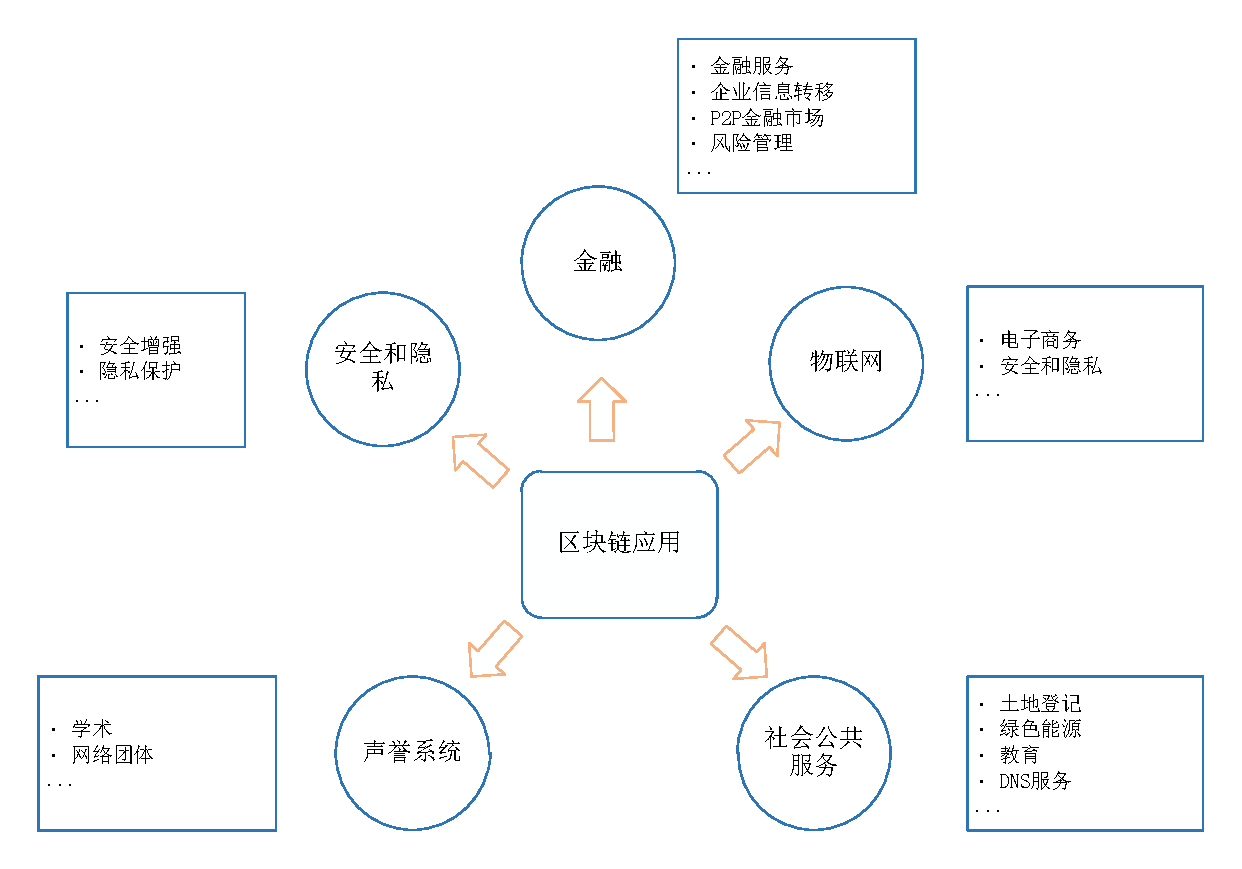
\includegraphics[width = 0.8\textwidth]{img/applications}
 	\caption{区块链典型的应用领域}\label{fig:applications}
\end{figure}

%from the use of blockchains appplication-driven analysis of applica... and a critical review of blockchai nand its current applications

%financial service
\subsubsection{金融}

区块链技术最受关注的应该是金融方面的应用,其中很大一部分原因是因为区块链作为比特币的底层技术,其最开始衍生的相关应用都和密码货币相关。在2015年,已经有相关研究者讨论将区块链应用在银行当中\supercite{peters2015trends}。在16年微软和IBM也相继推出了自己的区块链平台,希望作为一种服务提供给传统的金融机构。同时,区块链在企业资产转移、P2p金融市场和分享管理上,都做出了相应的尝试。

\subsubsection{物联网}

物联网通过传感器将大量的设备连接在一起,其间通过传感器获取数据并自动的完成数据的交换,可以很适宜的将区块链应用到其中。如智能汽车、记录运输药物过程中的温度\supercite{bocek2017blockchains}、食品运输信息\supercite{schneider2017design}以及感知病人数据都是物联网和区块链相结合的一些尝试,不仅减少了制造商的成本,也让客户对相关商品信息更加放心,两方都能从中获益。一些研究者也对物联网和区块链的结合进行了探讨,\parencite{hardjono2016cloud}中提出了一个全新的物联网电子商务模型,基于区块链上智能合约来完成交易的自动化;同时使用区块链完成无需可信第三方认证的物联网构建,提升了物联网的安全和隐私。


\subsubsection{社会公共服务}

区块链也被广泛的应用在各种社会公共服务当中,其中最为典型的例子是土地登记,将土地的信息如物理状态和所有权放置在区块链上\supercite{survey2015blockchain}。区块链也被应用与加固互联网基础设施上面,如域名和身份的管理,Blockstack\supercite{ali2016blockstack}和NameCoin\supercite{loibl2014namecoin}就是将DNS服务建立在区块链上的尝试。同时,区块链也被用在如教育、能源、婚姻登记及税务系统构建\supercite{akins2014whole}等公共服务。

\subsubsection{声誉系统}

声誉是作为一个社区信任的衡量标准,可以通过其之前的行为和与社会的交互进行评判。Sharples等人提出了基于区块链的分布式教育信息声誉系统\supercite{sharples2016blockchain},用于记录各个教育机构和相关个人的声誉情况,任何相关的改变都可以很轻易的被检查到。\parencite{carboni2015feedback}中设计了一系列的投票写,将用户的反馈行为记录到区块链上,进而对服务供应商完成声誉评估。


\subsubsection{安全和隐私}

区块链技术同时也被用来巩固传统计算机相关服务的安全和隐私。Charles在2016年提出了一个名为BitAV的反恶意软件环境,用户在区块链上发布和查询病毒的相关信息,其改善了扫描速度并增强了系统的鲁棒性。就本文所述的PKI系统而言,也有很多方案被提出用于增强其安全性,如在\parencite{baldi2017certificate}中,将撤销的证书存储在区块链上,提供更加可靠的证书验证服务,可以避免传统OSCP中单点失效的问题。IKP\supercite{matsumoto2016ikp}方案利用以太坊智能合约,将PKI中证书相关的操作都转移到区块链上,记录证书的申请、签发以及吊销过程,让PKI中的各个步骤都是公开可审计的,此时区块链相当于是公开且不可篡改的日志服务器,供大家审计PKI系统中的所有操作。MIT Media Lab等人提出了名为MedRec\supercite{azaria2016medrec}的项目,利用区块链去中心化的特性来提升病人对自己医疗数据的管理权,完成对数据访问和共享的控制,使得用户隐私得到了进一步保障。




% 同样,PKI系统也是建立在中心化的体系结构之下的,同样可以通过区块链的去中心化特性带来更好的安全性。一些研究希望通过将区块链技术应用在PKI系统中,弥补现有体系中的一些缺陷,例如在\parencite{baldi2017certificate}中,将撤销的证书存储在区块链上,提供更加可靠的证书验证服务,可以避免传统OSCP中单点失效的问题。IKP\supercite{matsumoto2016ikp}方案利用以太坊智能合约,将PKI中证书相关的操作都转移到区块链上,记录证书的申请、签发以及吊销过程,让PKI中的各个步骤都是公开可审计的,此时区块链相当于是公开且不可篡改的日志服务器,供大家审计PKI系统中的所有操作。

% %blockstack?? or ETHIKS or CONIKS


% Certcoin\supercite{fromknecht2014decentralized}借鉴Namecoin实现了一个基于区块链的PKI系统,其通过默克尔哈希树来完成对身份信息的存储并通过Kademlia DHT完成快速查询。Nidaba\supercite{rystsovnidaba}则从分布式PKI的可扩展性和证书操作的代价出发,基于区块链提出了一套完整的架构;SCPKI\supercite{al2017scpki}利用web-of-trust模型以及以太坊上的智能合约,提出了一种去中心化且透明的方案,保证异常证书被签发时能够及时的被检测到。%turn a blcokchain into PKI


% %supply Chain
% 供应链是区块链应用中另外一个被广泛讨论的应用场景,利用区块链去中心化和不可篡改的特性,将供应链中相关信息记录到区块链上,可以为供应链增加透明度、信任、互操作性以及减少开销等好处。其中最为著名的应用是将区块链融入全球的物流运输,IBM和Maersk在2017年宣布通过区块链建立托运人、货运代理、海运承运人、港口和海关的网络;供应链涉及其它方面主要是食品和药物。

% %healthcare

% 医疗领域应作为区块链涉足的另外一个领域,其旨在利用区块链解决现有医疗系统中的互通性问题\supercite{mettler2016blockchain}。\parencite{yue2016healthcare}中提出基于区块链的医疗数据网关(HDG)方案,其中使用了私有区块链网络来存储医疗相关的信息,保证存储的用户数据不回被泄露。
% MIT Media Lab等人提出了名为MedRec\supercite{azaria2016medrec}的项目,利用区块链去中心化的特性来提升病人对自己医疗数据的管理权,完成对数据访问和共享的控制。


%IOT


%computer science




\section{本文研究工作和章节安排}


通过上述分析和说明,可以得知现有的PKI构建在一个中心化的层级模型之上,其中存在着一系列问题,其中最为核心的问题是现有的PKI系统需要对CA给予绝对的信任。本文将围绕这一问题对PKI系统进行分析和讨论,并对区块链技术进行介绍,给出一种基于区块链技术的解决方案。



%本文将对给出方案进行详细阐述,分析方案的安全性,

本文结构如下图所示\ref{fig:plan}:


\begin{figure}[htbp]
 	\centering
 	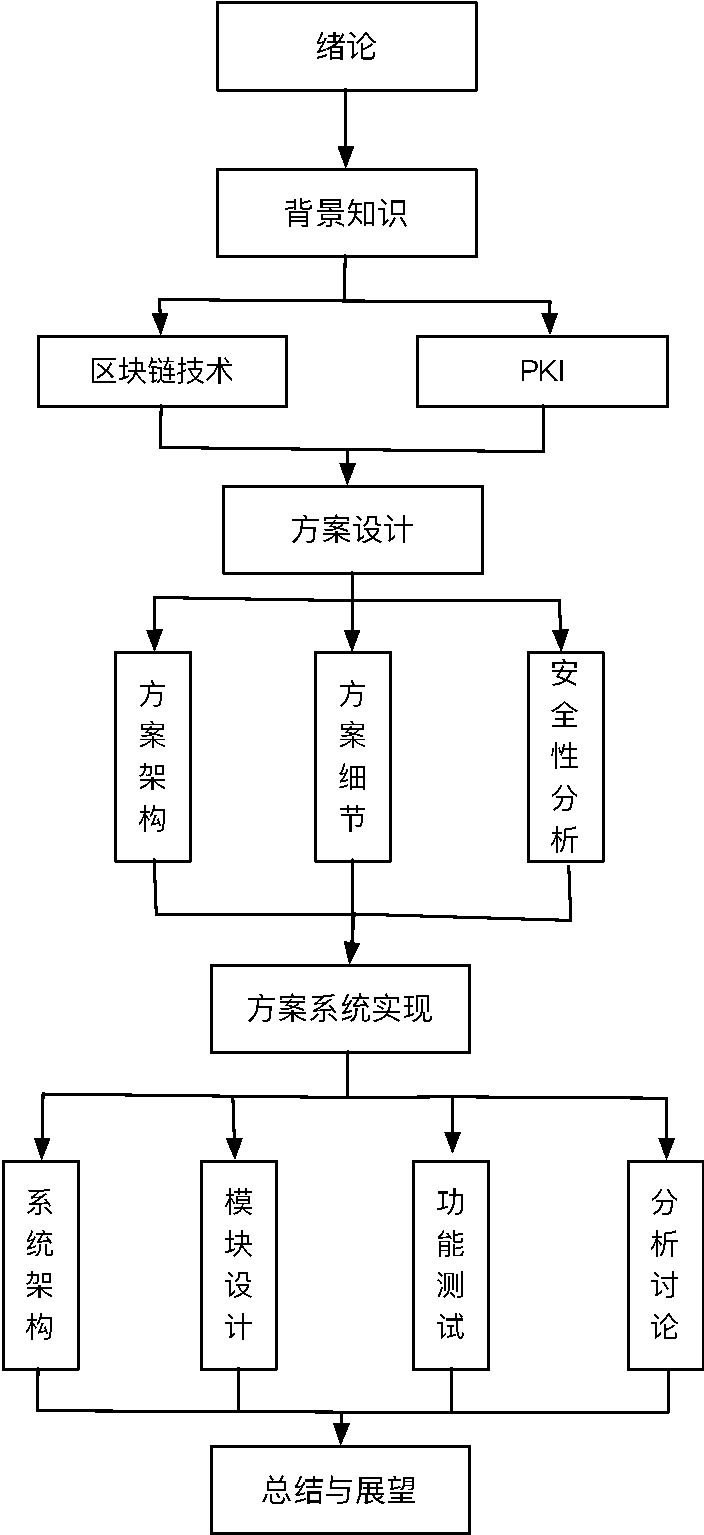
\includegraphics[scale=0.7]{img/plan}
 	\caption{文章结构}\label{fig:plan}
\end{figure}

% 本论文的章节结构如下:

第一章:论文绪论,介绍本文的研究背景和研究意义,给出PKI的研究现状以及区块链的应用现状,提出研究的问题,并简要说明本文的组织结构。

第三章:介绍PKI的相关知识,介绍PKI系统和证书,给出PKI系统中存在的问题和已有的改善措施;其后介绍区块链技术的基本知识,包括比特币、共识和智能合约等概念,并介绍区块链的应用场景

第三章:介绍一种基于区块链的命名实体鉴权方案的设计,首先给出方案的概述,描述方案设计到角色和工作流程,然后对方案进行详细阐述,并对方案的安全性进行分析。

第四章:阐述本文给出方案的一种系统实现,给出系统设计和模块设计,根据设计对系统进行实现,并进行系统功能性测试和相关分析。

第五章:对本文提出的方案进行总结,并对未来的工作提出展望。



% vim:ts=4:sw=4
